\documentclass[12pt,a4paper]{article}
\usepackage[]{listings}
%packages used
\usepackage[english]{babel}
\usepackage[margin=1in,  left=1.25in]{geometry} %margins
\usepackage{pslatex}%Times new roman font
\usepackage{graphicx}%for images
\usepackage{float}
%\usepackage{fancyhdr}
%\pagestyle{fancy}
%\fancyfoot{}

%beginning of document
\begin{document}
%declaration page
%\thispagestyle{empty}
\pagenumbering{roman} 
\begin{titlepage}
  \begin{center}
    \vspace*{1cm}

    \textbf{\Huge Single cycle CPU  report}

    \vspace{0.5cm}

         
    \vspace{1.5cm}

    \textbf{\large Chang Zihao \\20206018\\\large Cui Yuxuan\\20206019}

    \vfill
         

         
    \vspace{0.8cm}
  


         
\end{center}
\end{titlepage}


\newpage
%table of contents
\tableofcontents
\thispagestyle{empty}

\newpage
\pagenumbering{arabic}
\setcounter{page}{1}

\section{Introduction}

Lab3 is required to design a Single-cycle CPU.
A single-cycle CPU processes an instruction per every single clock cycle.

\subsection{Data Path}

\begin{enumerate}
\item Fetch the instruction at the address in PC.
\item Decode the instruction.
\item Execute the instruction.
\item Update the PC to hold the address of the next instruction. 
\end{enumerate}

\subsection{Control-Single}

\begin{enumerate}
\item Operation to be performed by ALU.
\item Whether register file needs to be written.
\item Signals for multiple intermediate multiplexors.
\item Whether data memory needs to be written. 
\end{enumerate}

% Lab 3 is intended to give you hands-on experience in designing the simplest form of a modern microprocessor, whose operations are conducted within a single clock cycle. 
% Based on the concepts and skills you have acquired through Lab 1 and Lab 2, you are now ready to implement a single-cycle CPU. 
% Through this lab assignment, you will have gained an in-depth understanding on the fundamentals of designing a CPU microarchitecture.  

% \subsection{Backgrounds}

% A CPU is composed of two types of units, which are the control units and data units. 

% \subsubsection{Control Path \& Data Path}
% A control path consists of multiple control units, which “controls” the data path of the processor (e.g., ALUs, memory) how to respond to the instruction that is fetched to the processor. 
% Likewise, a data path is a collection of functional units such as arithmetic logic units (ALUs) or multipliers, that perform data processing operations, registers, and buses. 
 
% \subsection{Single-cycle CPU}

% A single-cycle CPU processes an instruction per every single clock cycle. 
% At every single clock cycle, the singlecycle CPU must perform Instruction Fetch (IF), Instruction Decode (ID), Execute (EX), Memory operation (MEM), and Write Back (WB) stages of a single instruction, so the architectural states are updated as the instruction “instructs” the CPU. 
% The IF stage is to fetch the instruction that the Program Counter (PC) points to in the instruction memory. 
% The ID stage is to decode the fetched instruction, figure out which operations are required to carry out, which is defined by the Instruction Set Architecture (ISA). 
% The EX stage is where primitive operations (e.g., add, multiply, bit-wise operations) as well as memory address calculations are performed. 
% The MEM stage is to perform memory operations (e.g., load, store) on specified address by the instruction. 
% The WB stage is to update the architectural states of the processor; the values of registers or memory are updated as a result of executing the instruction. 
% The exact control and data path are shown in Fig. 1, which is the MIPS version of a single cycle CPU design. 


\newpage

\section{Design}

As the Description of TB file mentioned, We do not need to implement memory and register ourselves.
So we design the path to connect them together.
Then we have to design some necessary modules.

\subsection{Module design}

\subsubsection{ALU module}

ALU has been designed in lab1.
But this time we need to modify the ALU slightly.
At the beginning, I took out the Cout alone to deal specifically with branch instructions
It works, but not necessary.
So I put the Cout back and cancel it.


\subsubsection{PC module}

The PC is a state element that holds the address of the current instruction. 
It is updated at the end of every clock cycle.

\subsubsection{add module}

The adder is responsible for incrementing the PC to hold the address of the next instruction.
It takes two input values, adds them together, and outputs the result

\subsubsection{HALT module}

HALT is used to halt the program when a specific condition is met.
The terminate condition is ($RF\_ RD1 = 0x0000000c$) when the received instruction is 0x00008067. 
HALT needs to set 1 when the terminal condition is met.

\subsubsection{Sign extend module}

Single extend module is used to increase the number of bits of a binary number while preserving the number's sign and value. 

\subsubsection{MUX module}

Mux, a data selector, which was used to select which the single will be output.

\newpage

\section{Implementation}

The whole circuit was shown below.

\begin{figure}[H]
  \centering
  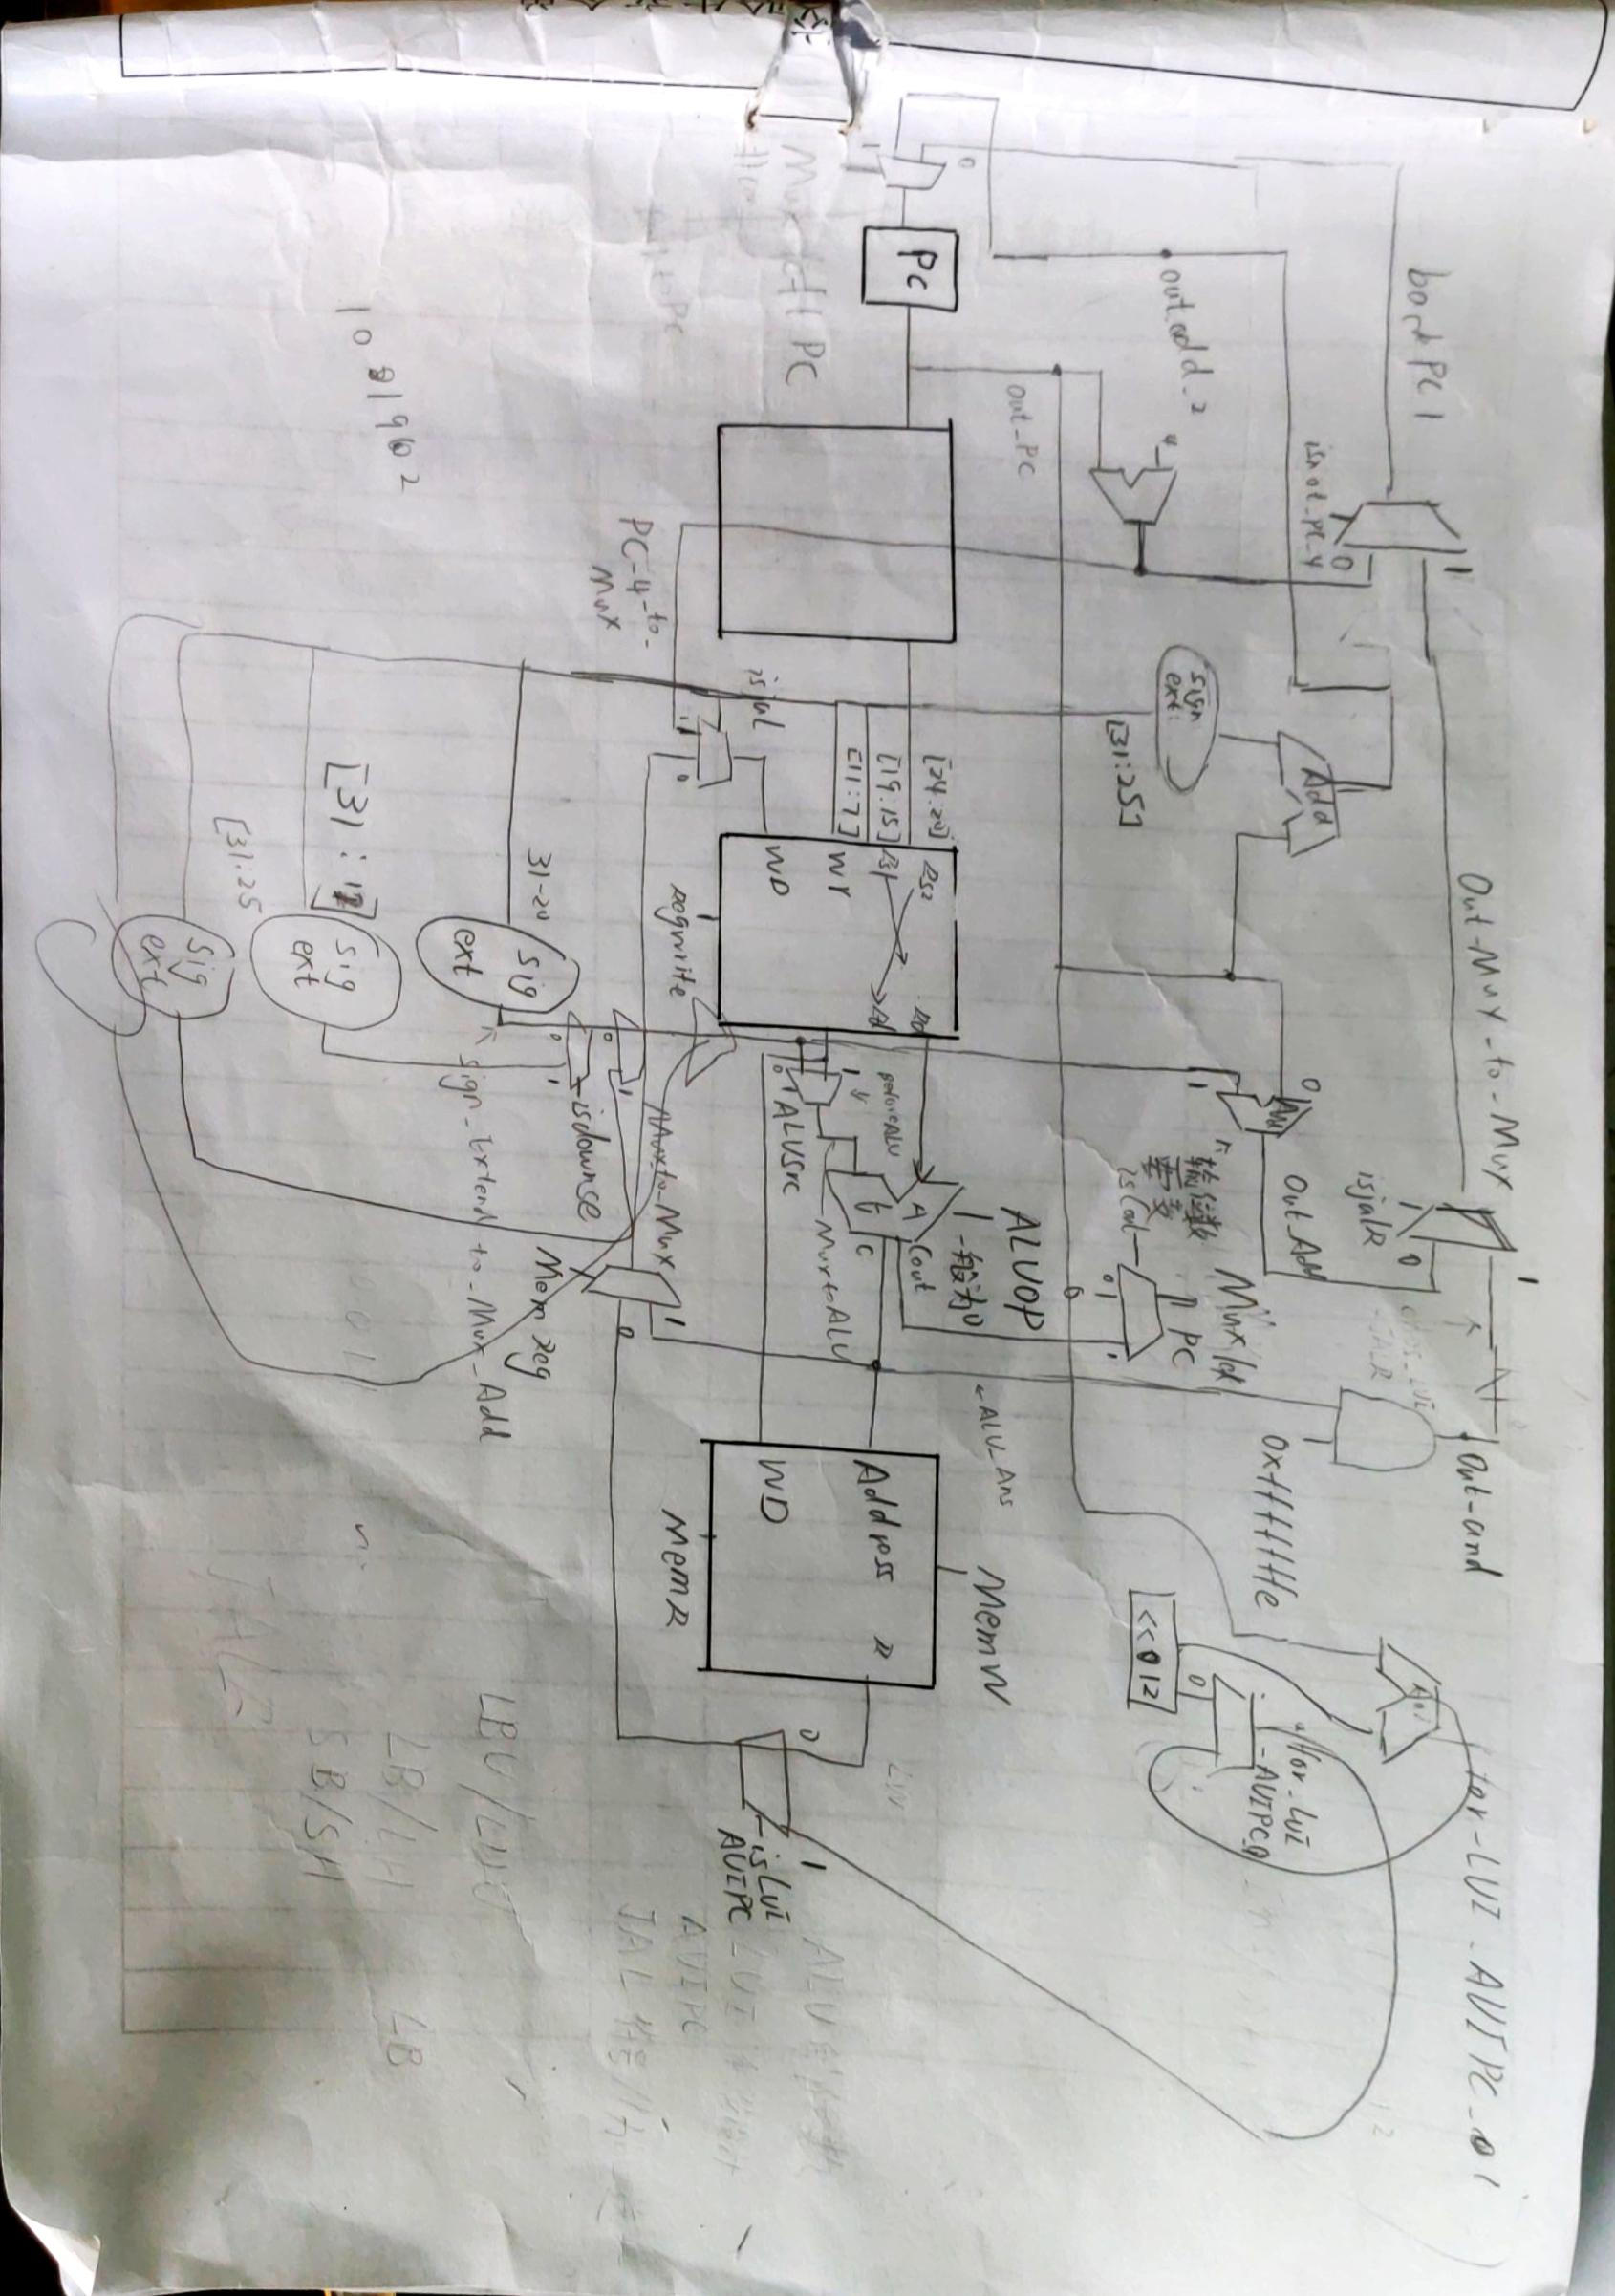
\includegraphics[height=6in, angle=90]{Lens.jpg}
  \end{figure}

There might be something different with the circuit.
Such as, I cancel the cout output.
\newpage

\section{Evaluation}

I pass all the test in the testbench folder.

\begin{figure}[H]
  \centering
  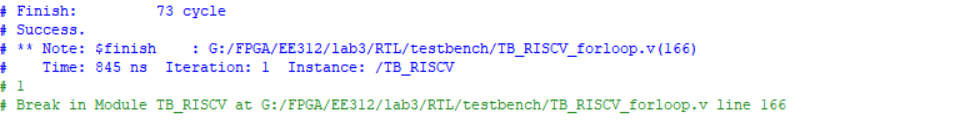
\includegraphics[height=1in]{1.PNG}
  \end{figure}

\begin{figure}[H]
  \centering
  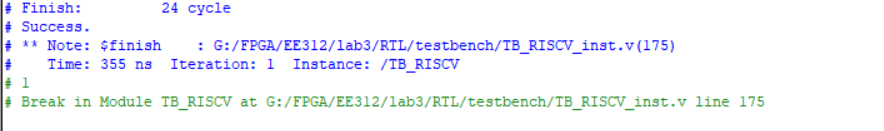
\includegraphics[height=1in]{2.PNG}
  \end{figure}

  \begin{figure}[H]
    \centering
    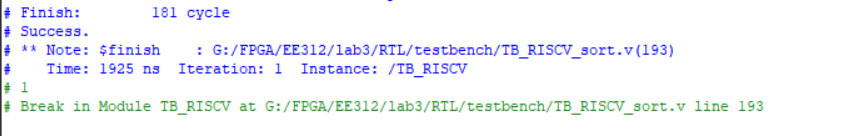
\includegraphics[height=1in]{3.PNG}
    \end{figure}

% We first encountered some problems in understanding the meaning of the question, 
% but in the end by looking at the test code, 
% we thoroughly understood the meaning of the question.
% And at last, we pass all the test and finished the whole project.
% I hope that future projects will give enough time to think and complete the code.

\section{Conclusion}

The single-cycle CPU is easy to design but have some disadvantages.
Such as the clock cycle will be determined by the longest possible path, which is not the most common instruction. 

\end{document}
